
\chapter{Homework 1}
Show work in all sections. I suggest you utilize MATLAB/Octave 
for developing functions and plotting (although other languages 
[Python, R] are allowed). Please include axes labels, units, and 
titles on all plots. Plot logs vertically (y axis is depth). 
Please place all results in a single word/pdf file for review. 
Essay answers should be complete. Please include all functions 
and scripts in the writeup. You are allowed to discuss the homework 
assignment with others but every student must turn in their own 
report and independently develop scripts/codes.

%%%%%%%%%%%%%%%%%%%%%%%%%%%%%%%%%%%%%%%%%%%%%%%%%%%
%                  1. Part-1
%%%%%%%%%%%%%%%%%%%%%%%%%%%%%%%%%%%%%%%%%%%%%%%%%%%
\section{Part 1: Understanding Bounding Models.}
You are given a small data set consisting of velocity measurements on 
54 different clastic samples at pressures 5, 10, 20, 30, and 40 MPa. 
The file is Data.mat located on the Canvas site. 
It contains a matrix of the data (Data) and structure that lists 
what is in each column of the matrix (Column-Names).

% \subsection{Problem 1}

%%%%%%%%% T-1 %%%%%%%%%%
\begin{problem}{1}
    Use the Data.mat file from the Canvas site. 
    Select the water-saturated Vp (Column 6), Vs (Column 7), 
    density, porosity, and clay content data for 30 and 40 MPa (Column 5). 
    Discard the rest of the data. After you have the data for 30 
    and 40 MPa, divide them into two parts: 1 for clean sandstone 
    (Clay < 20\%) and shaley sandstone (Clay >= 20\%).
\end{problem}

\begin{solution}
    \begin{figure}[H]
        \centering
        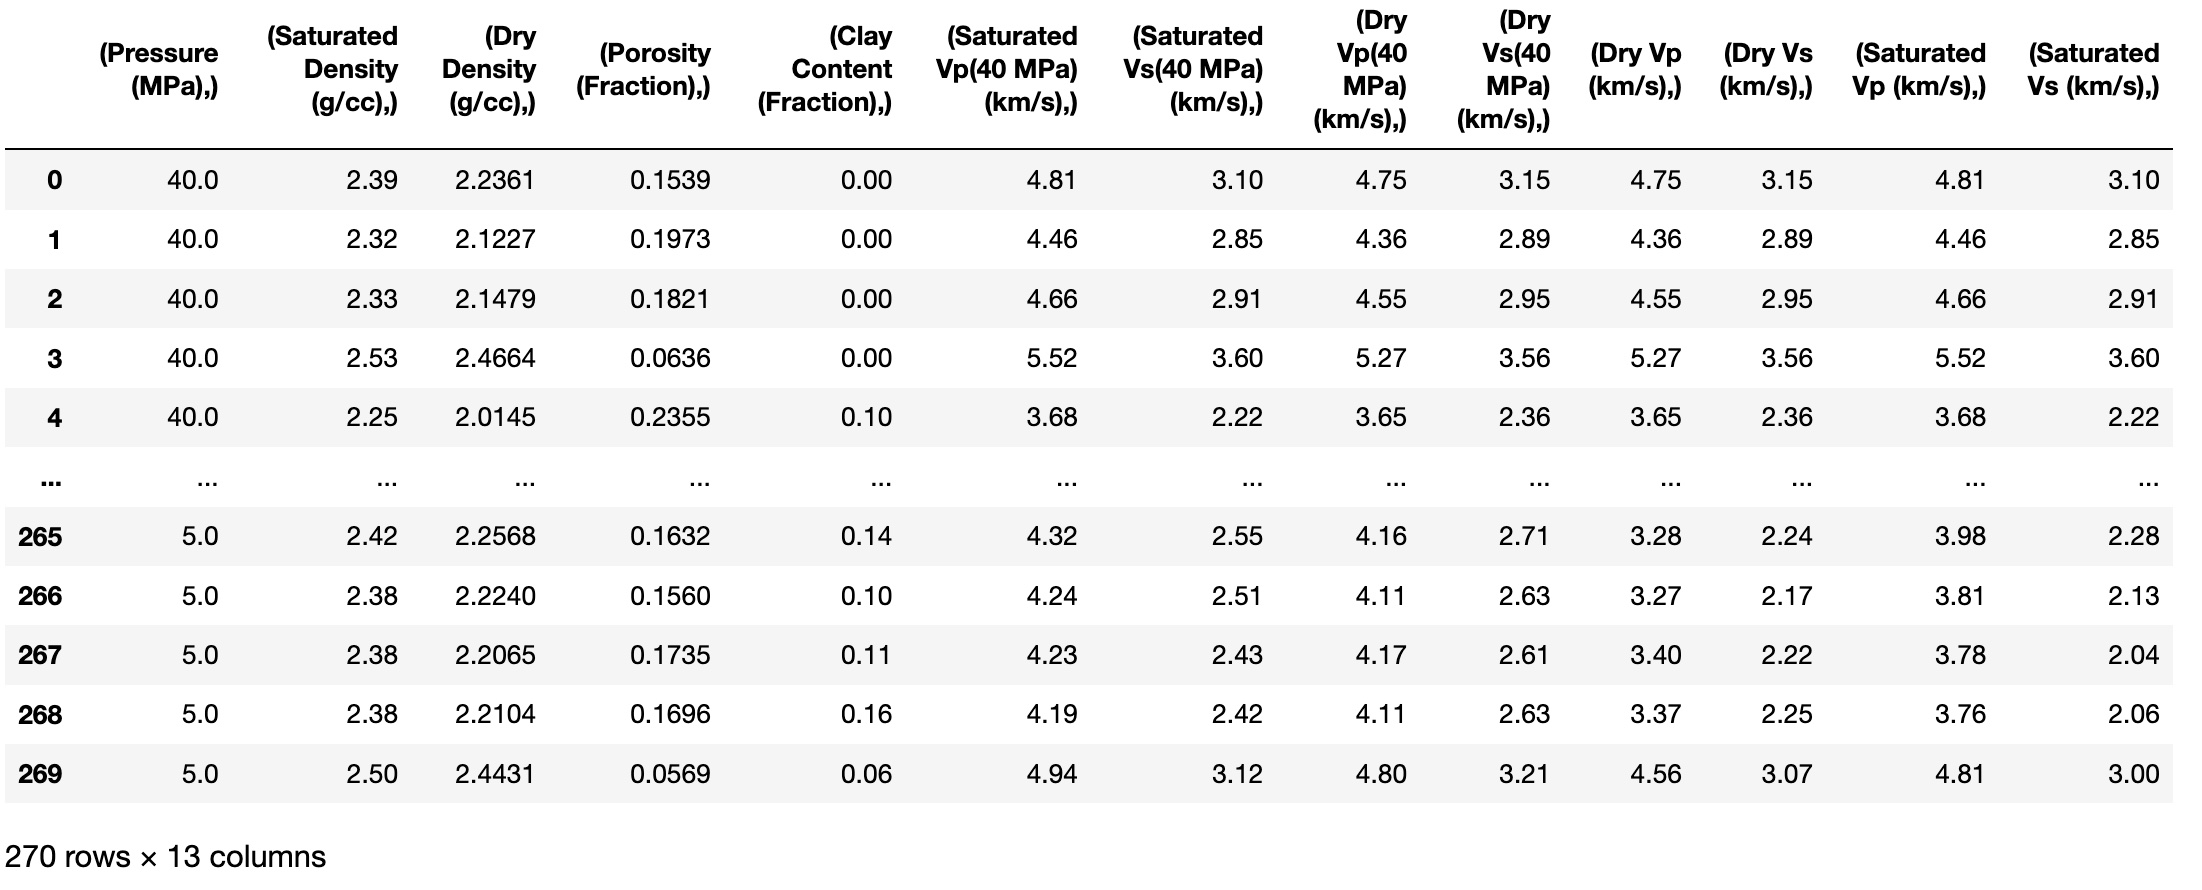
\includegraphics[width=0.7\textwidth]{figures/homework-1/p1-problem-1.jpg}
        \caption{Data.mat}
        \label{fig:p1-problem-1}
    \end{figure}
    After reading the Data.mat showing in figure ~\ref{fig:p1-problem-1}, I select the useful data and divide it into 2 parts: clean sandstone and shaley sandstone.
    Please check the scripts for details.
\end{solution}



%%%%%%%%% T-2 %%%%%%%%%%
\begin{problem}{2}
    (2a) Plot the clean sand data, specifically, bulk modulus as a function of porosity. On the same axes, plot Voigt-Reuss bounds of bulk modulus as a function of porosity for a mixture of quartz and water. Label the curves.
    (2b) On the same axes as (2a), plot upper and lower Hashin-Shtrikman bounds of bulk modulus as a function of porosity. Label the curves.
    (2c) On a $2^{nd}$ set of axes, repeat (2a) except for shear modulus.
    (2d) Repeat (2b) except for shear modulus.
\end{problem}

\begin{solution}

Use the following formulas to transform Vp, Vs and density to bulk and shear modulus.
\begin{align}
    K & = \rho * ({V_p}^2 - 4/3 * {V_s}^2)\\
    u & = \rho  * {V_s}^2
    \label{equ:K-u-modulus}
\end{align}

Then calculate Voigt-Reuss bounds and Hashin-Shtrikman bounds for a mixture of quartz and water.
The final results showing in figure ~\ref{fig:p1-problem-2}.

\begin{figure}[h]
    \centering
    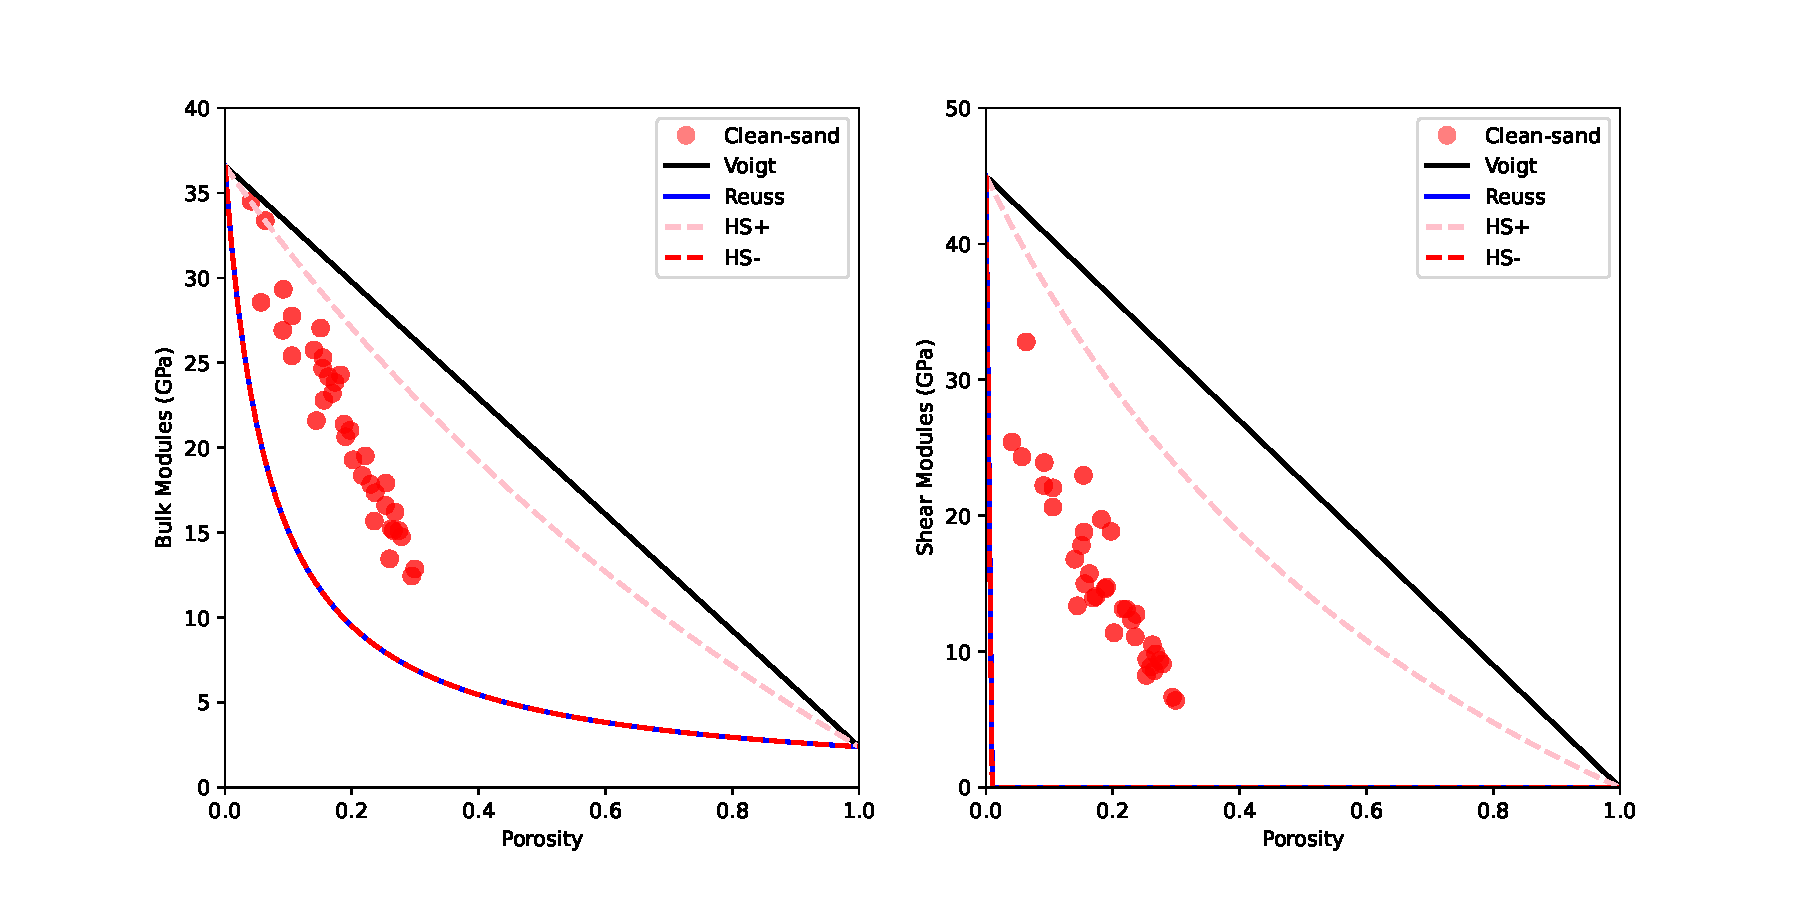
\includegraphics[width=0.8\textwidth]{figures/homework-1/p1-problem-2.pdf}
    \caption{Bulk and shear modulus of clean sandstone data}
    \label{fig:p1-problem-2}
\end{figure}
\end{solution}


%%%%%%%%% T-3 %%%%%%%%%%
\begin{problem}{3}
    (3a) On a 3 rd set of axes, plot the clean sand data, this time Vp as a function of porosity. On the same axes, plot the Voigt-Reuss bounds of Vp as a function of porosity. Label the curves.
    (3b). On the same axes as 3a) plot upper and lower Hashin-Shtrikman bounds of Vp as a function of porosity. Label the curves.
    (3c) On a 4 th set of axes, repeat 3a) except for Vs.
    (3d) Repeat 2b) except for Vs.
\end{problem}

\begin{solution}

    Calculate Voigt-Reuss bounds and Hashin-Shtrikman bounds for a mixture of quartz and water.
    Then use the following formulas to transform bulk, shear modulus and density to Vp and Vs.
    \begin{align}
        V_p & = \sqrt{\frac{K+ 4/3 u}{\rho} } \\
        V_s & =  \sqrt{\frac{u}{\rho} }
        \label{equ:Vp-Vs}
    \end{align}
    
    The final results showing in figure ~\ref{fig:p1-problem-3}.
    \begin{figure}[h]
        \centering
        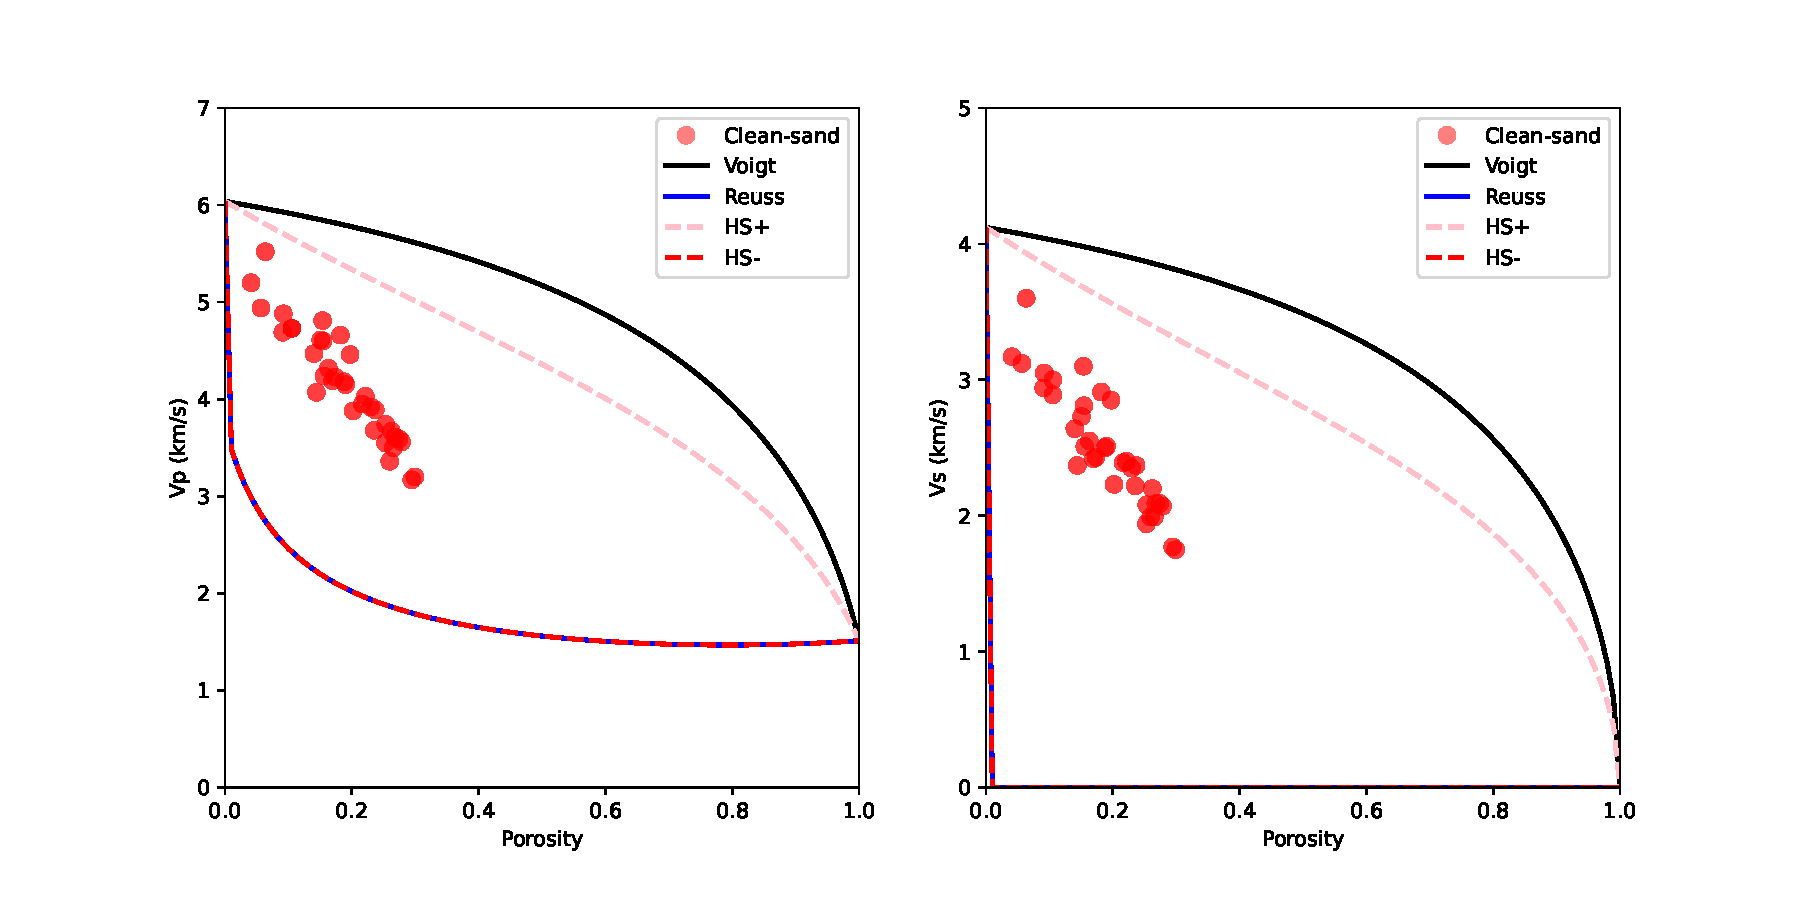
\includegraphics[width=0.8\textwidth]{figures/homework-1/p1-problem-3.pdf}
        \caption{Vp and Vs of clean sandstone data}
        \label{fig:p1-problem-3}
    \end{figure}
\end{solution}



%%%%%%%%% T-4 %%%%%%%%%%
\begin{problem}{4}
    Repeat problems 2 and 3 using the shaley sands. For the shaley sandstones, the amount of clay content in the solid mixture is a free parameter, so you must choose how much clay content to use in the bounds. You will still mix a fluid and a solid. The solid, however, is a combination of two minerals (quartz and clay). Mix mineral moduli using the Voigt-Reuss-Hill approach. When you have the mixture of the solids, that is the new 0 porosity end member value for the bounds. Use Table 1 as necessary.
\end{problem}

\begin{solution}

    I choose the fraction ratio of $\frac{quartz}{quartz+clay} $ to be 0.7 
    and use Voigt-Reuss-Hill approach to calculate the mix-modulus of quartz and clay.
    The final results showing in figure ~\ref{fig:p1-problem-4}.
    \begin{align}
        M_{VRH} & = \frac{M_V+M_R}{2}  \\
        M_V & =  \sum_{i = 1}^{N}  f_i*M_i \\
        \frac{1}{M_R} & =  \sum_{i = 1}^{N} \frac{f_i}{M_i}
        \label{equ:hill}
    \end{align}

    \begin{figure}[H]
        \centering
        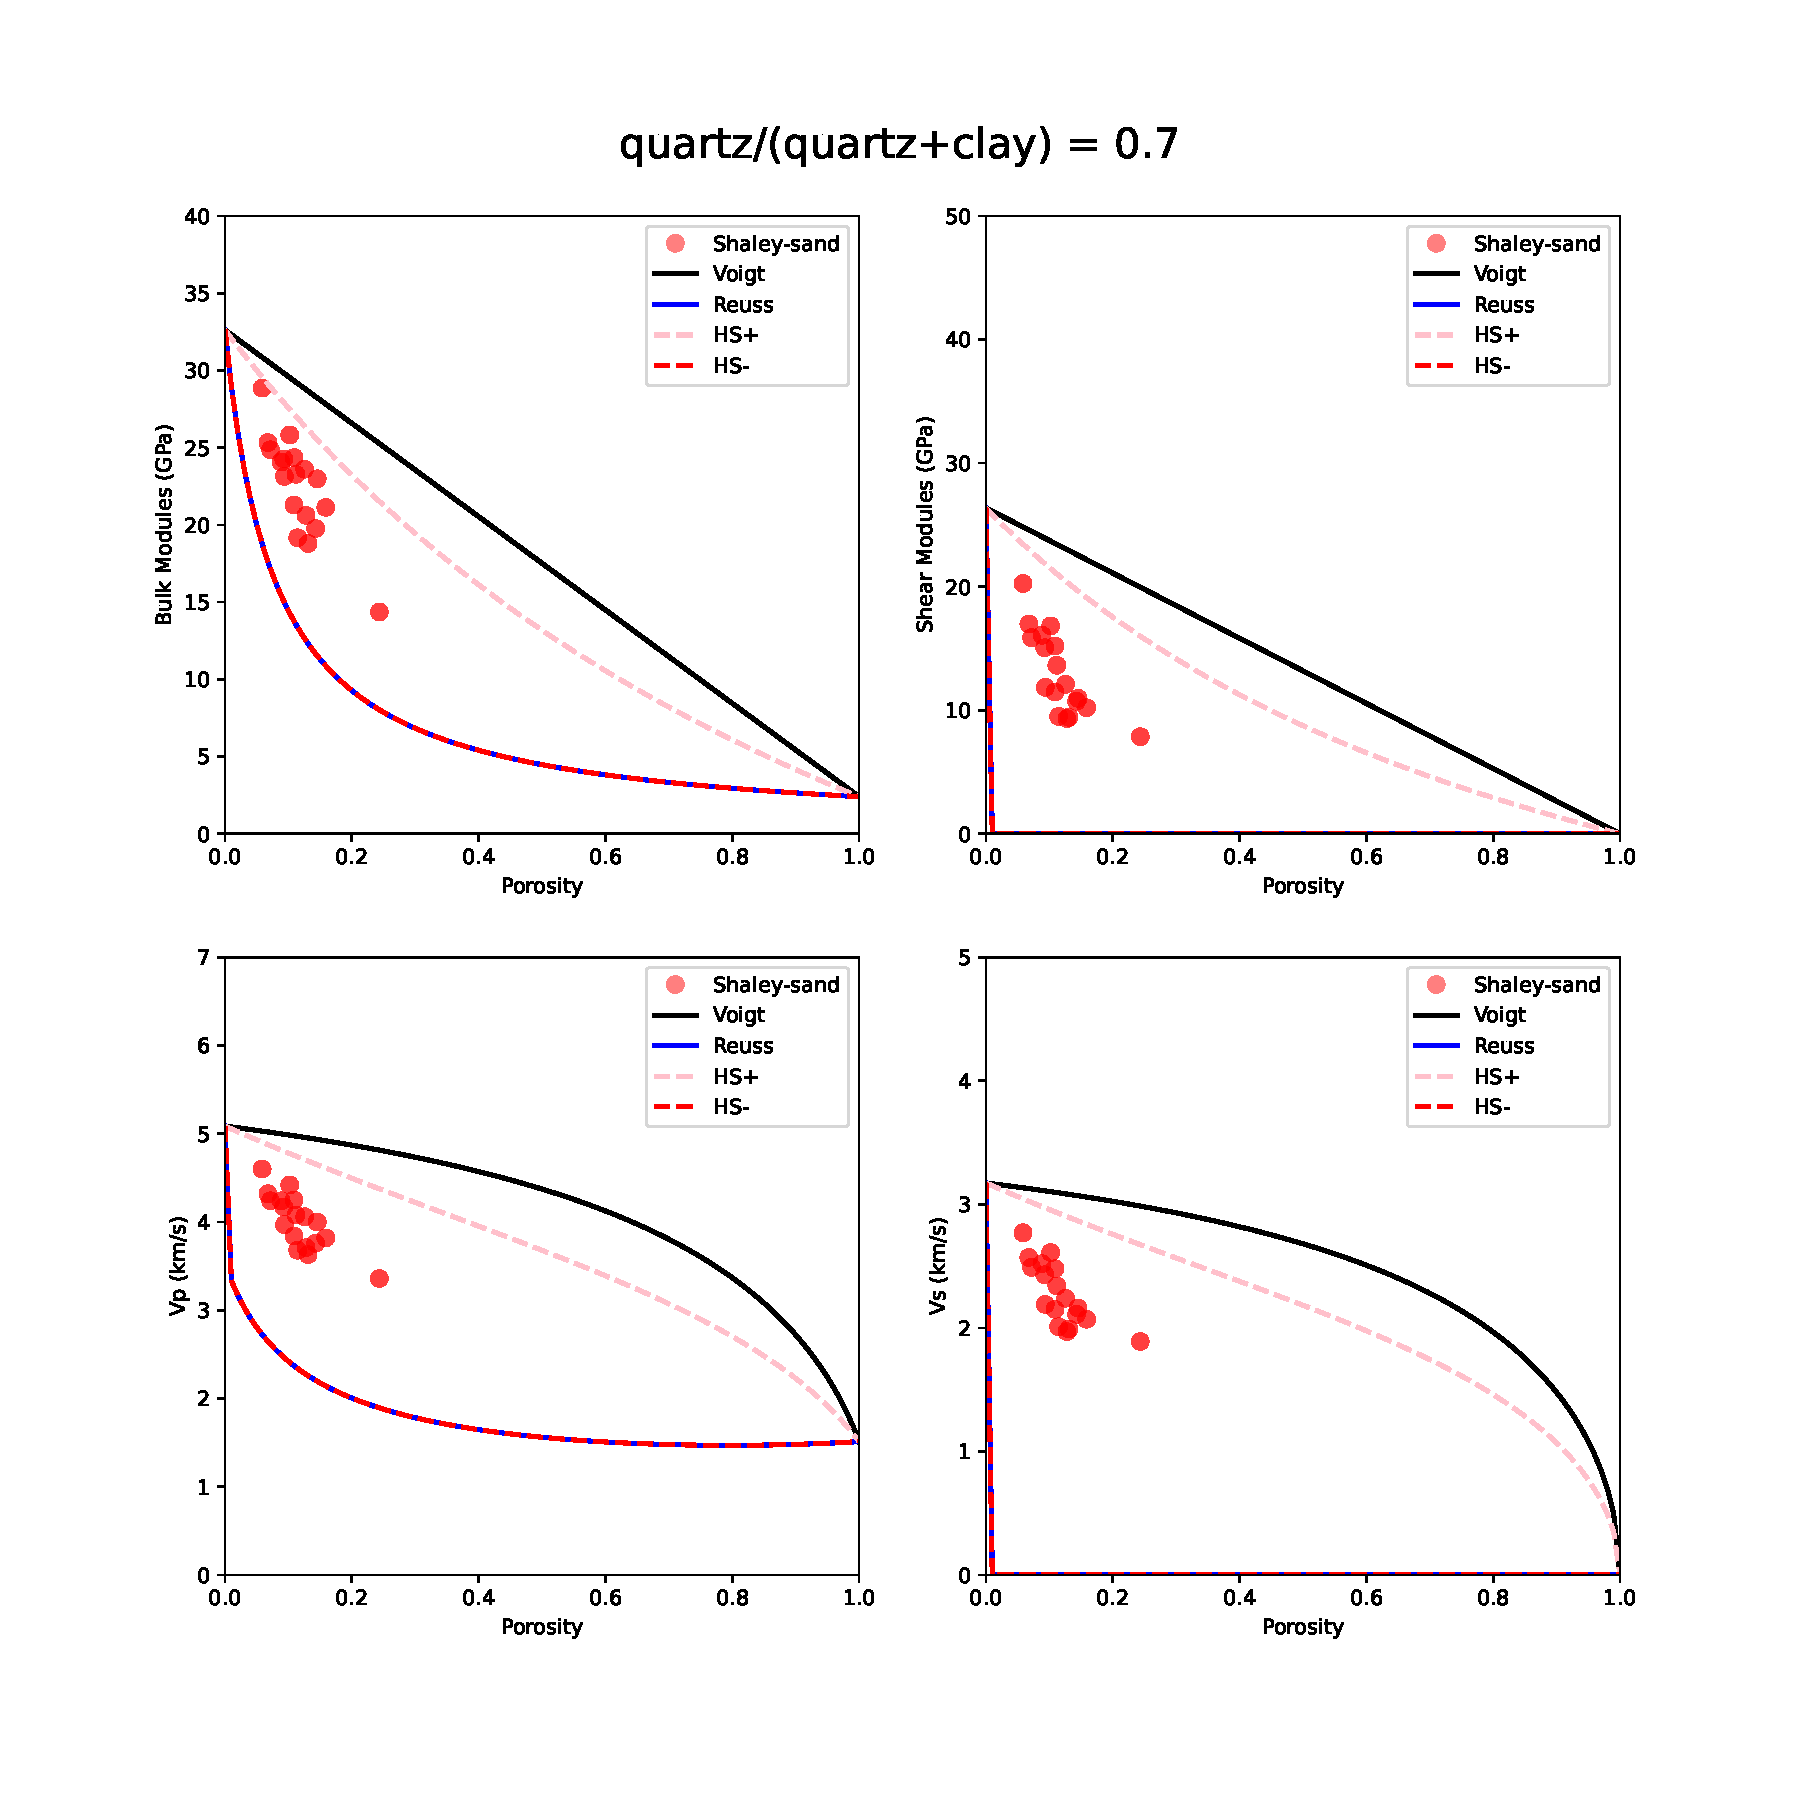
\includegraphics[width=0.8\textwidth]{figures/homework-1/p1-problem-4.pdf}
        \caption{Shaley sandstone data}
        \label{fig:p1-problem-4}
    \end{figure}
\end{solution}


%%%%%%%%% T-A %%%%%%%%%%
\begin{problem}{A}
    What are the geometric interpretations of the Voigt-Reuss and Hashin-Shtrikman bounds?
\end{problem}

\begin{solution}

    The Voigt bound is sometimes called the isostrain average because it gives the 
    ratio of the average stress to the average strain when all constituents are 
    assumed to have the same strain.
    \begin{figure}[H]
        \centering
        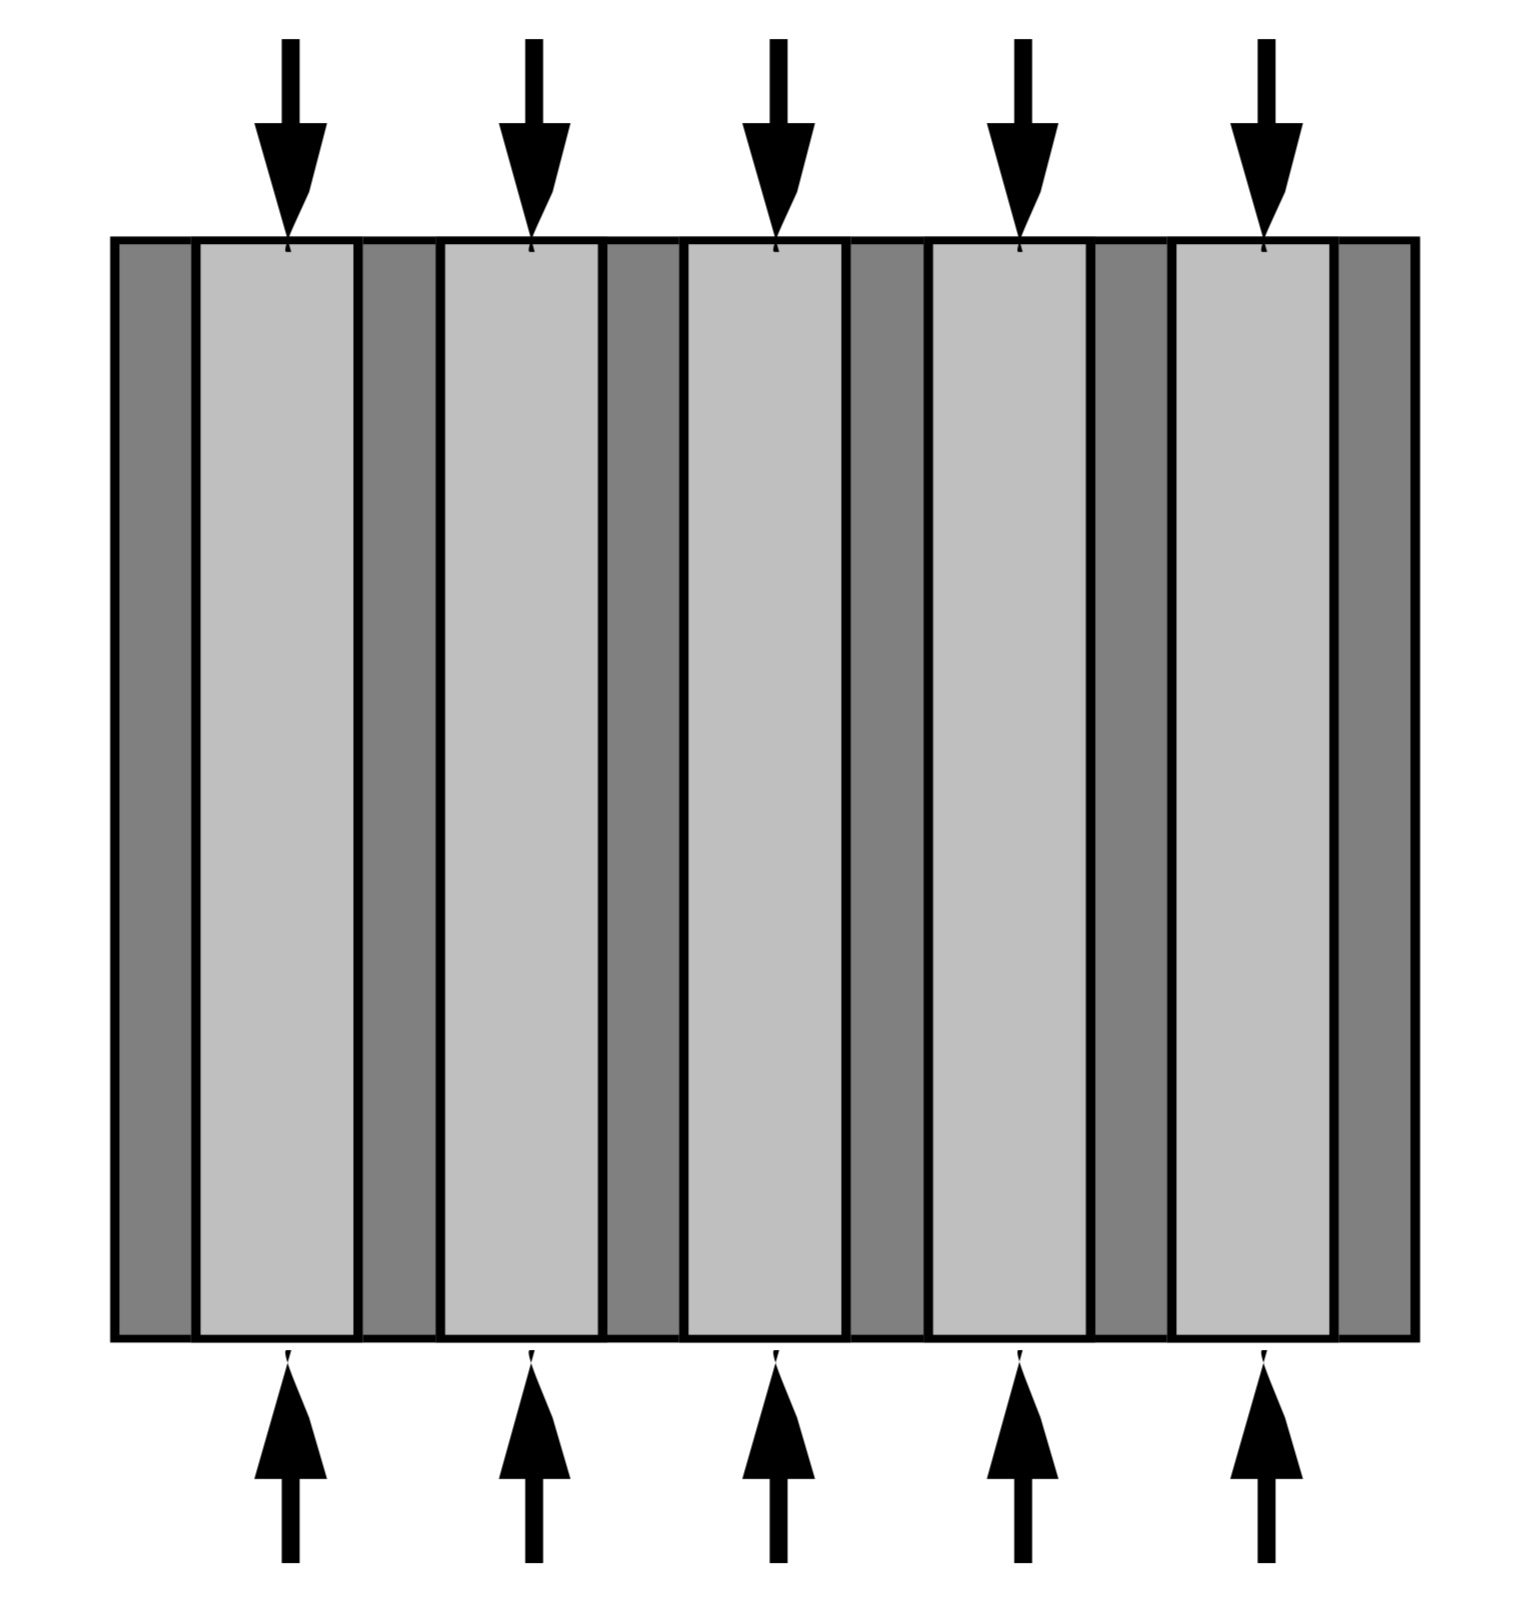
\includegraphics[width=0.3\textwidth]{figures/homework-1/Voigt-geometric.jpg}
        \caption{Voigt Geometric}
        \label{fig:Voigt-geometric}
    \end{figure}

    The Reuss bound is sometimes called the isostress average because it gives the 
    ratio of the average stress to the average strain when all constituents are 
    assumed to have the same stress.
    \begin{figure}[H]
        \centering
        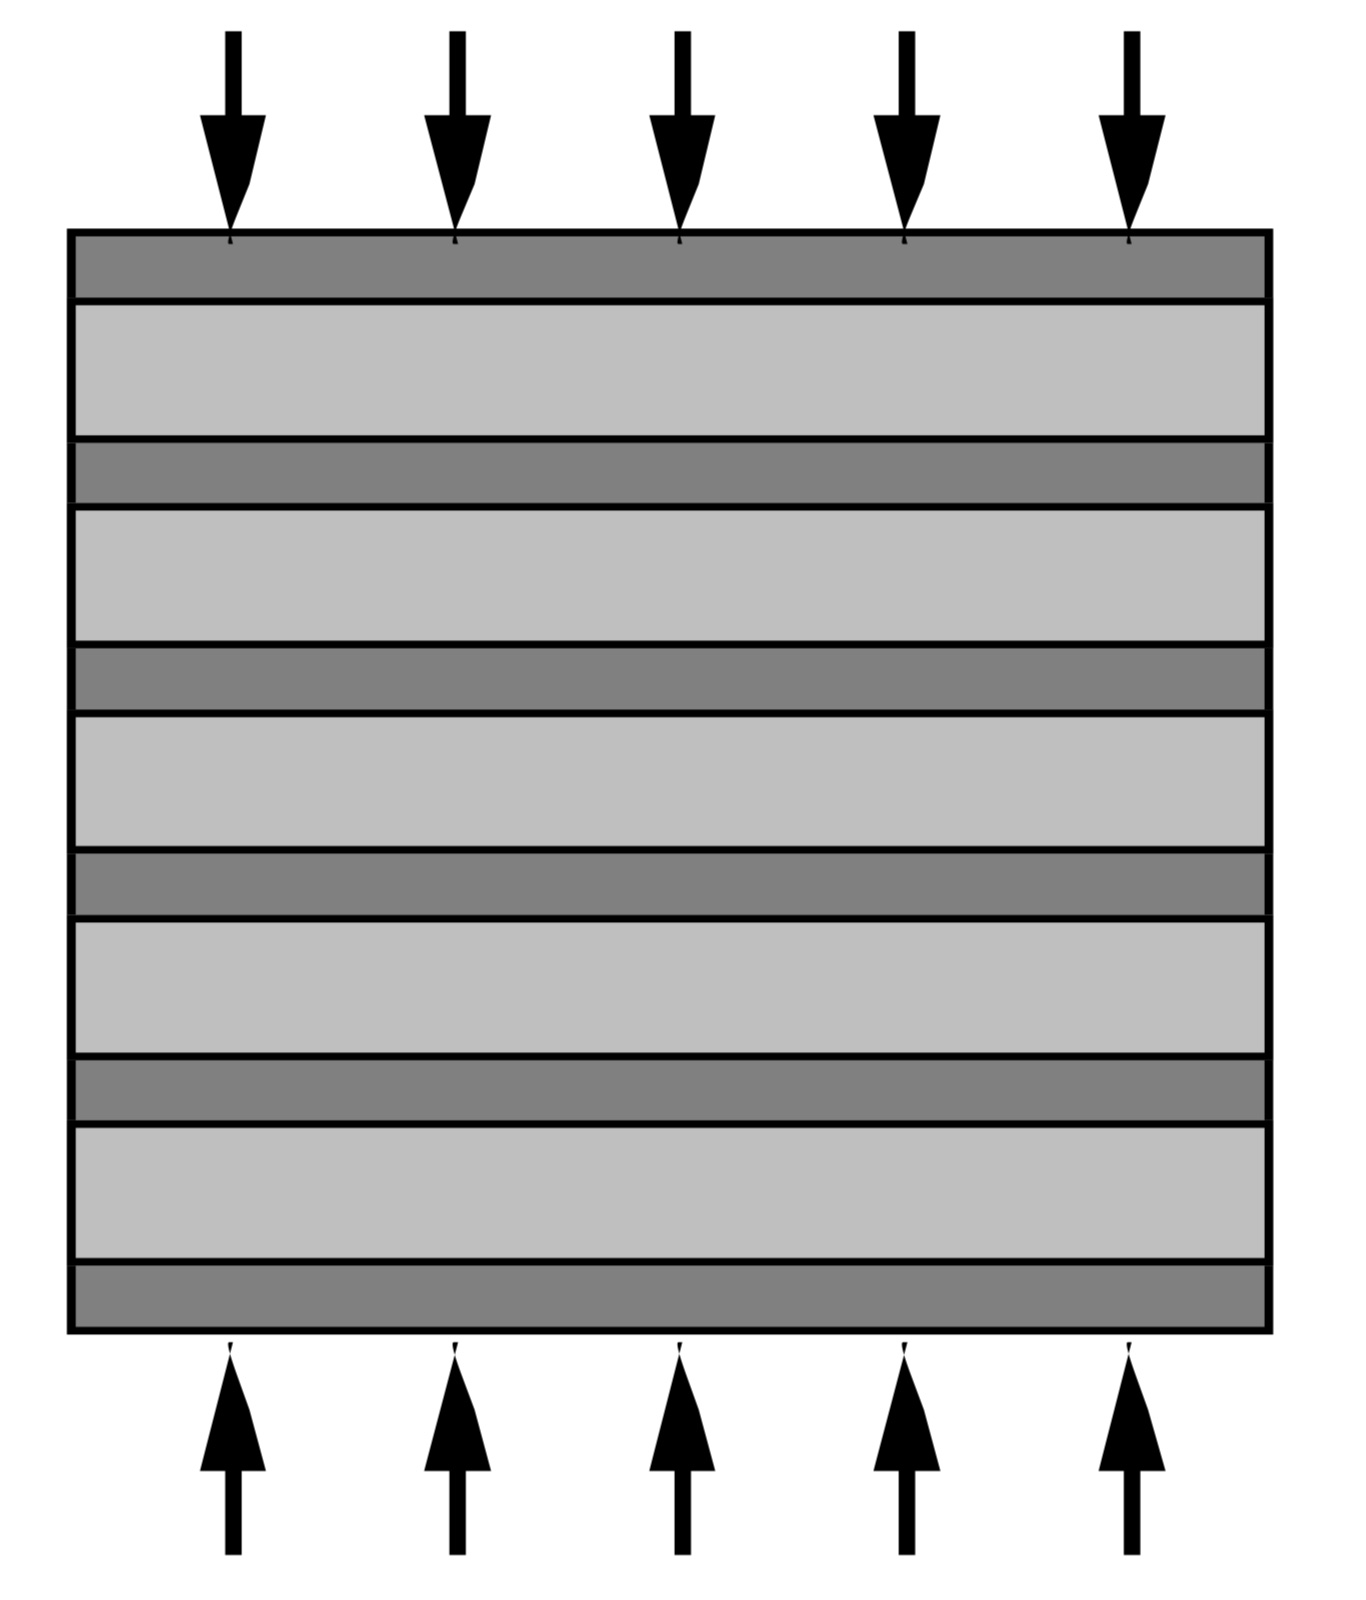
\includegraphics[width=0.3\textwidth]{figures/homework-1/Reuss-geometric.jpg}
        \caption{Reuss Geometric}
        \label{fig:Reuss-geometric}
    \end{figure}

    For Hashin-Shtrikman model, the space is filled by an assembly of spheres of material 2, each surrounded by a shell of material 1.
    The upper bound is realized when the stiffer material forms the shell; 
    the lower bound is realized when it is in the core. 
    The physical interpretation implies a very wide distribution of sizes of the 
    coated spheres such that they fill all the space.
    \begin{figure}[H]
        \centering
        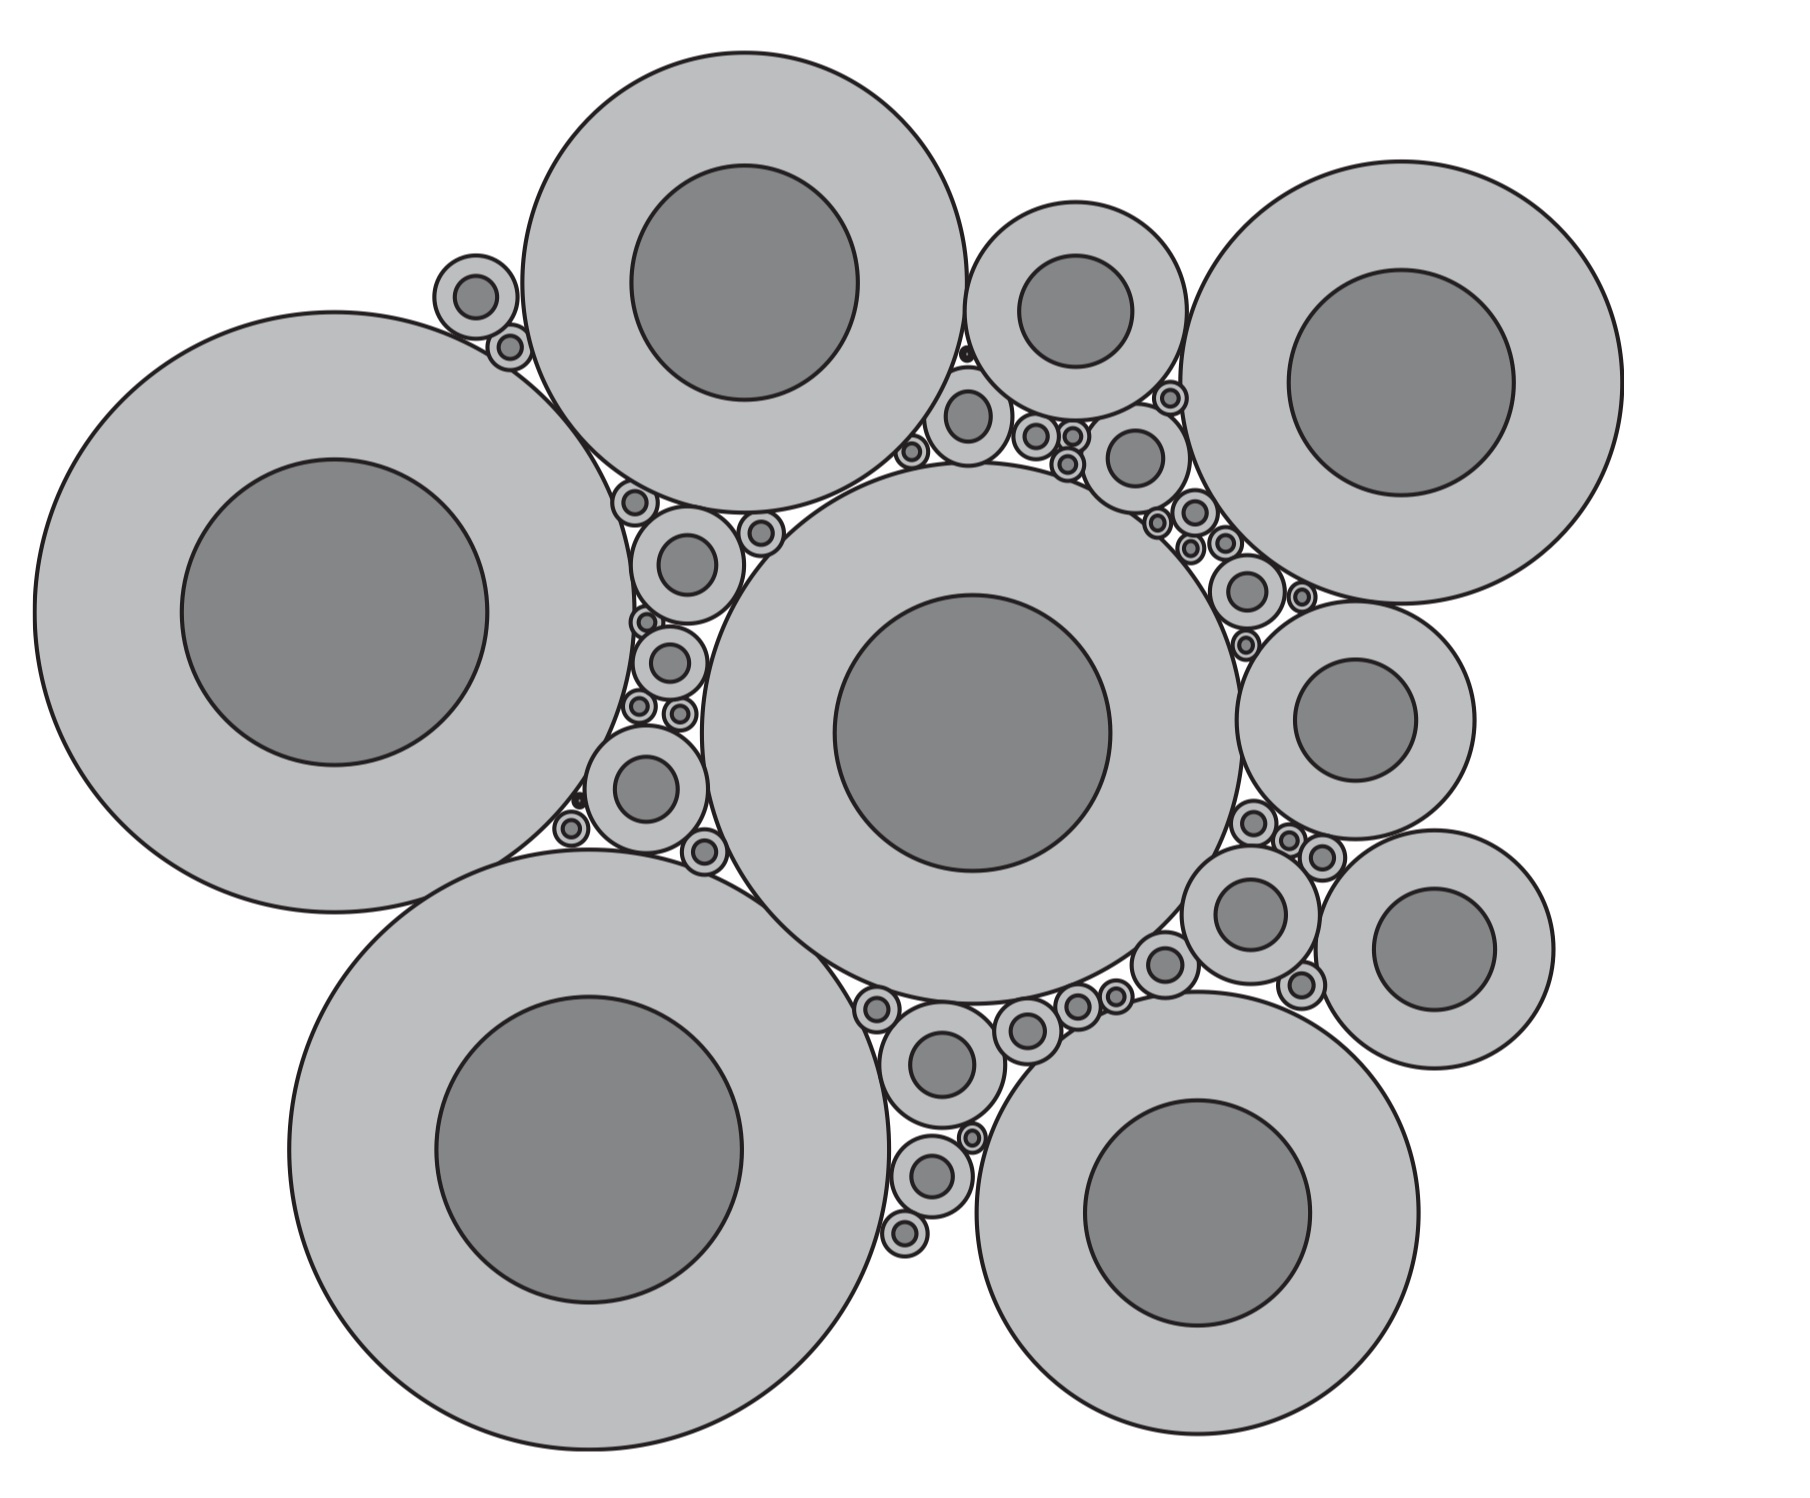
\includegraphics[width=0.5\textwidth]{figures/homework-1/Hashin-Shtrikman-geometric.jpg}
        \caption{Hashin-Shtrikman Geometric}
        \label{fig:Hashin-Shtrikman-geometric}
    \end{figure}
\end{solution}


%%%%%%%%% T-B %%%%%%%%%%
\begin{problem}{B}
    What are the geometric interpretations of the Voigt-Reuss and Hashin-Shtrikman bounds?
\end{problem}

\begin{solution}

    Voigt bounds is iso-strain and Reuss bounds is iso-stress.
\end{solution}



%%%%%%%%% T-C %%%%%%%%%%
\begin{problem}{C}
    What are the geometric interpretations of the Voigt-Reuss and Hashin-Shtrikman bounds?
\end{problem}

\begin{solution}
    Sediments with a layered structure are suitable for iso-stress bound interpretation.
    Because laminar system with strain applied perpendicular to lamination
\end{solution}



%%%%%%%%% T-D %%%%%%%%%%
\begin{problem}{D}
    What would happen to the effective mineral moduli if a mixture of 50\% quartz and 50\% feldspar was used instead of clay and quartz? Look up what the moduli for feldspar are (more than one set exists), and state which one you use to answer this question.
\end{problem}

\begin{solution}

    We find the bulk modulus is $37.5 GPa$, the shear modulus is $15 GPa$, and the density is $2.62 g/cc$ for feldspars.
    I find that all the bounds curves are moved up a little with the right end point is the fixed point.
    \begin{figure}[H]
        \centering
        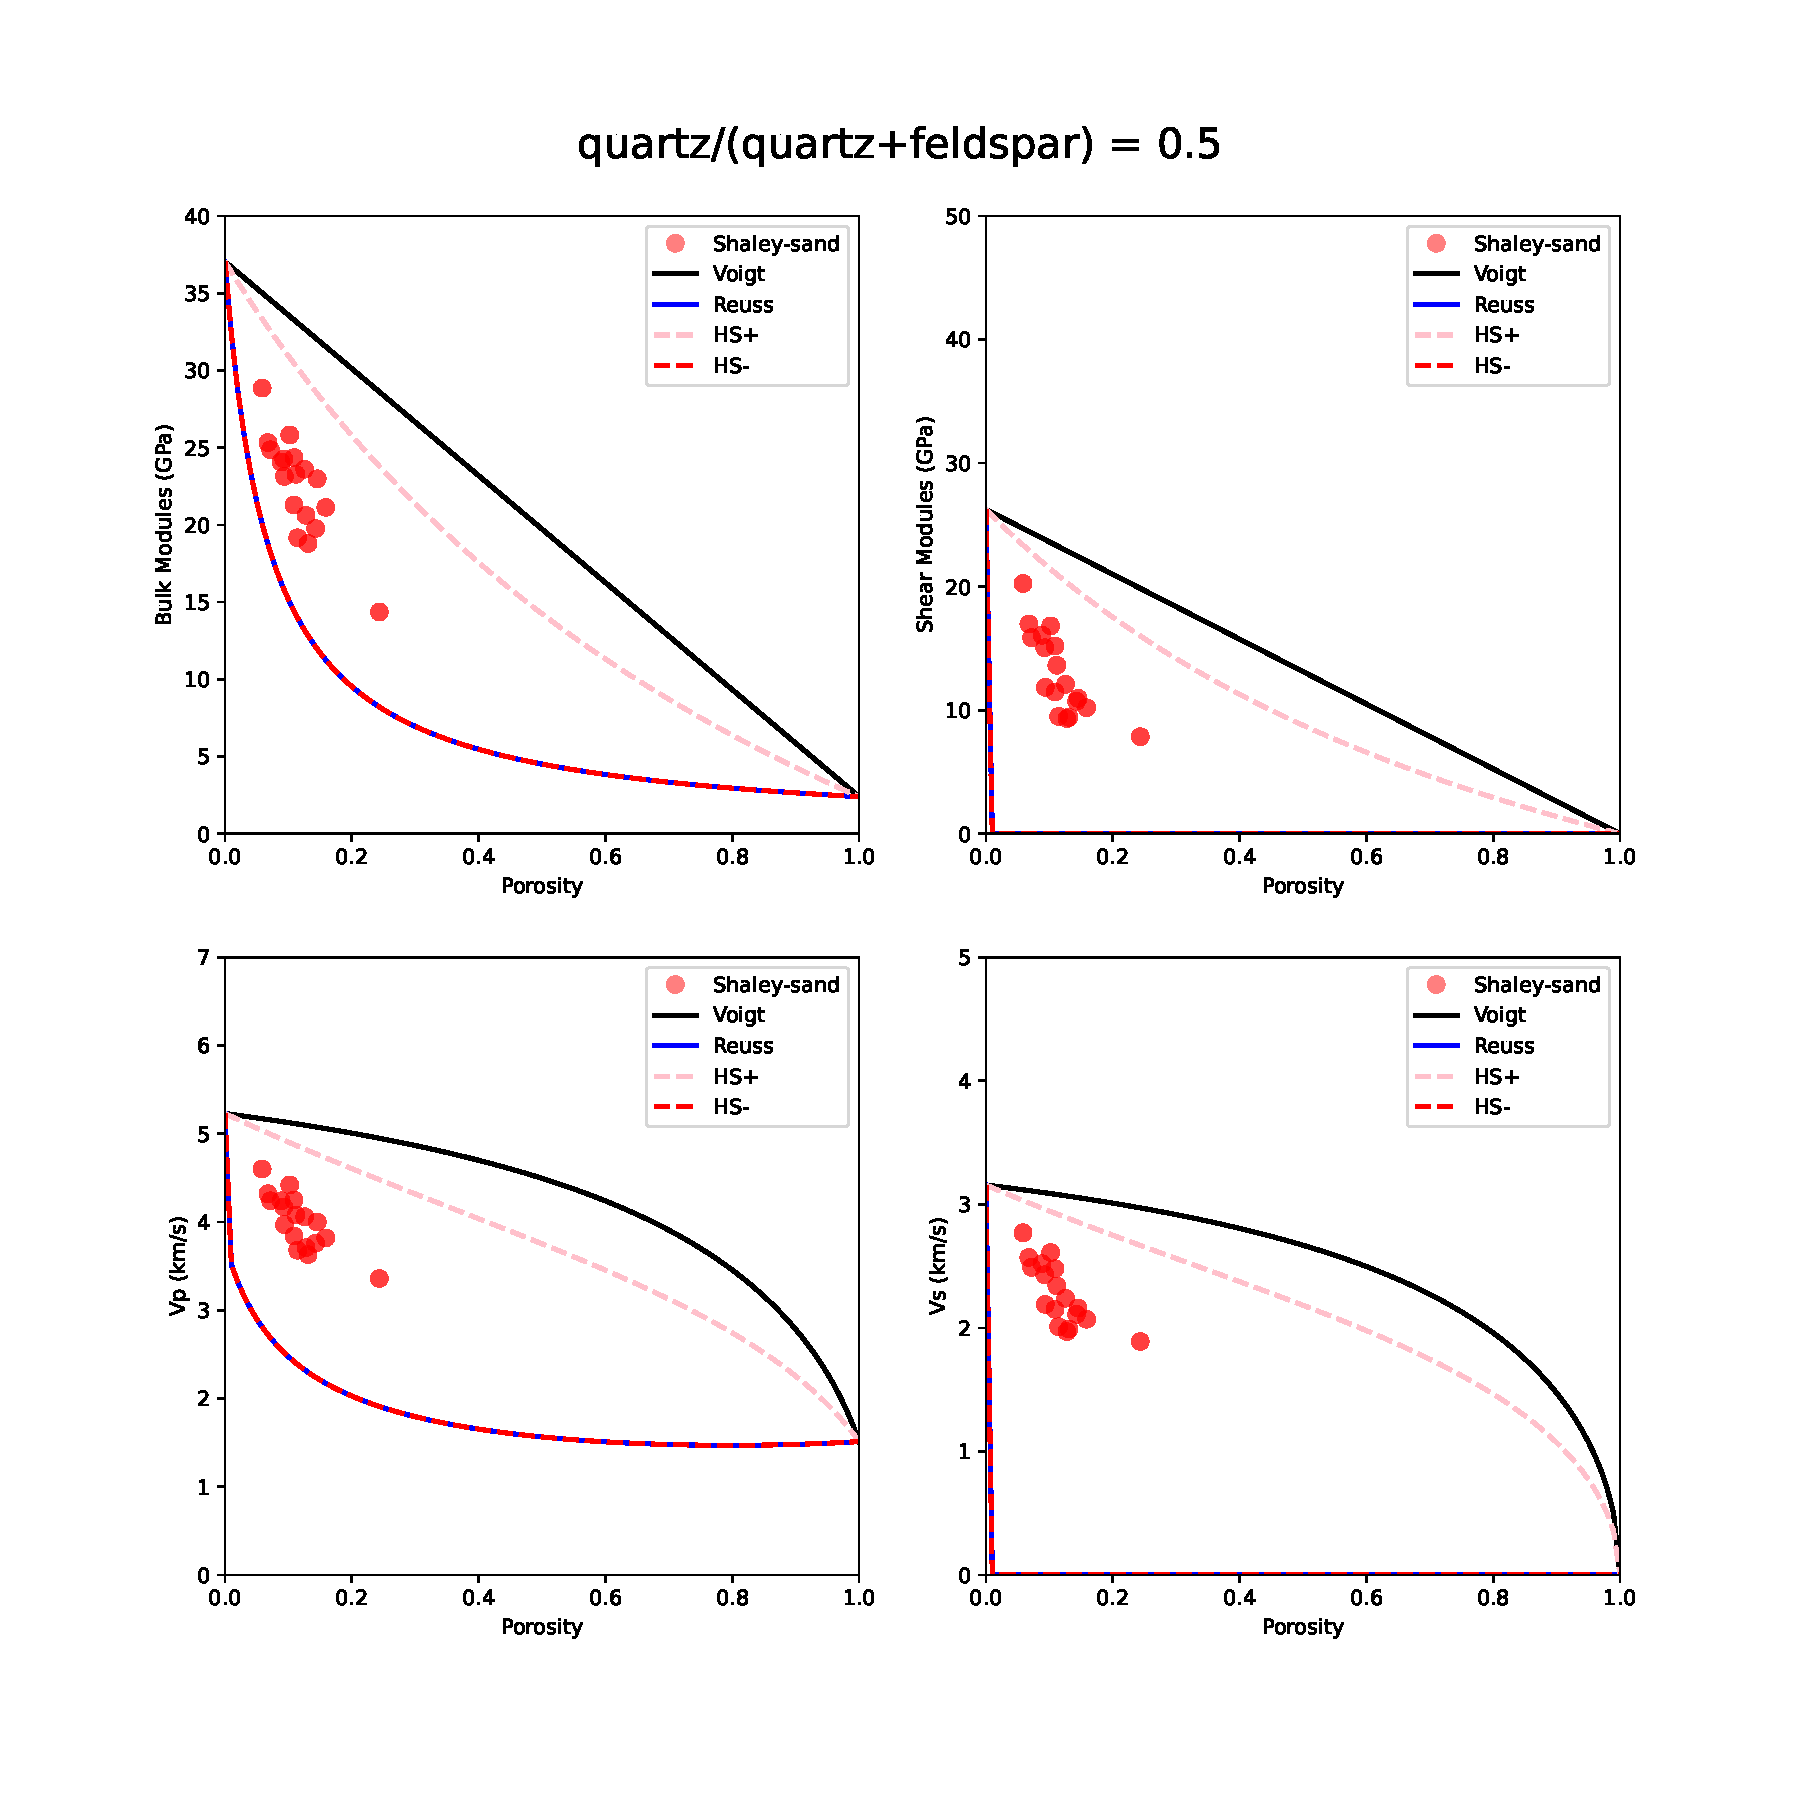
\includegraphics[width=0.8\textwidth]{figures/homework-1/p1-problem-d.pdf}
        \caption{A mixture of 50\% quartz and 50\% feldspar}
        \label{fig:p1-problem-d}
    \end{figure}
\end{solution}


%%%%%%%%% T-E %%%%%%%%%%
\begin{problem}{E}
    For the geometric interpretations of the H-S bounds, what possible depositional and/or diagenetic situations might approximate these two interpretations?
\end{problem}

\begin{solution}

    For the elastic moduli of mudrocks, consisting of a porous clay matrix mixed with quartz are actually well described using the lower HS bounds.
    The upper bound is realized when the stiffer material forms the shell.

\end{solution}












%%%%%%%%%%%%%%%%%%%%%%%%%%%%%%%%%%%%%%%%%%%%%%%%%%%
%                  2. Part-2
%%%%%%%%%%%%%%%%%%%%%%%%%%%%%%%%%%%%%%%%%%%%%%%%%%%

\section{Part 2}
This problem will provide you with an opportunity to experiment with Gassmann fluid substitution applied to a geologic CO 2 dataset from a past sequestration experiment in East Texas. On the Canvas site, you will find a text file called integratedLogSetV1.dat. This file contains the following important columns harvested from a sequence of logging runs.
The reservoir interval of concern is from depths of 5055 – 5072 ft, wireline depth.
Use these data for this problem. Use the ‘load’ function to read in the data. There are 7 columns in the file, and each column and its units are labeled in the top row of the text file. The well data contain two zones that produce gas. The task is to use fluid substitution for several different scenarios.


%%%%%%%%% T-1 %%%%%%%%%%
\begin{problem}{1}
    Use Gassmann’s model and determine the dry frame modulus (Kdry) from the sonic logs for the reservoir interval (depths above). Assume full brine saturation and quartz as the grain mineral. Remember to keep consistent units in calculations (MKS).
\end{problem}

\begin{solution}

    Firstly read the 'integratedLogSetV1.dat' showing below.
    \begin{figure}[H]
        \centering
        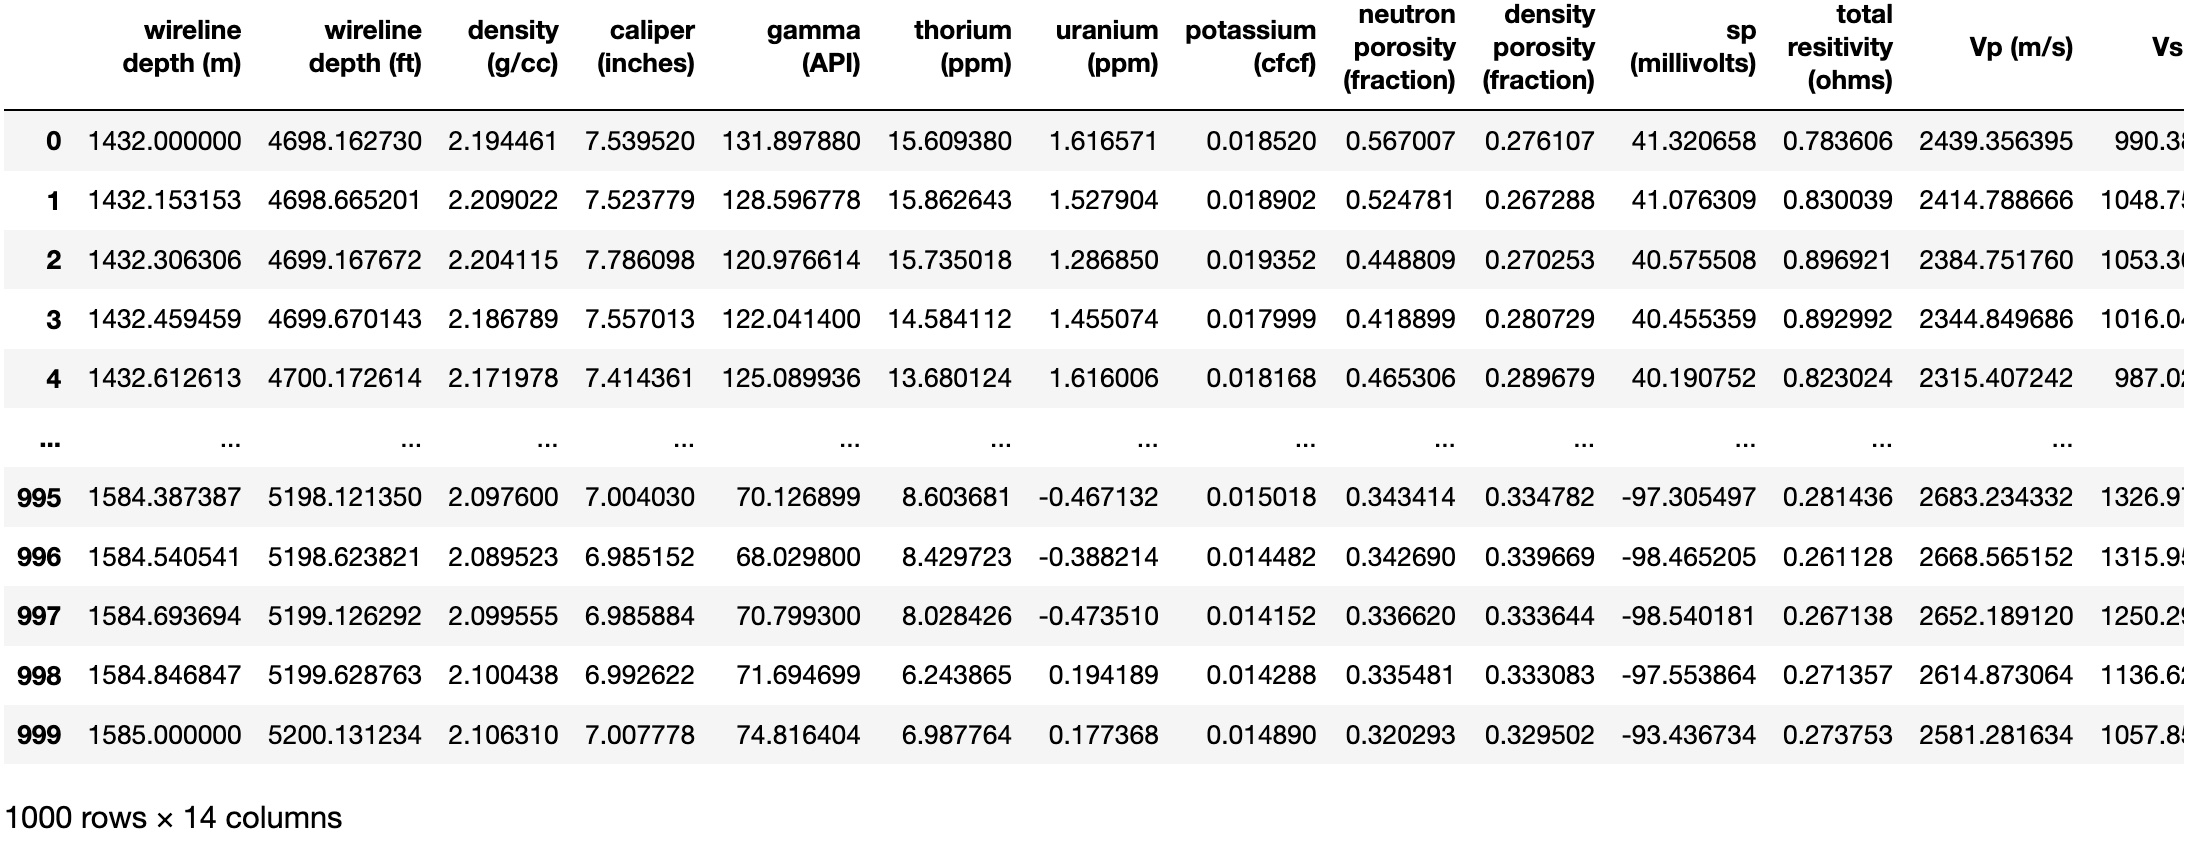
\includegraphics[width=0.9\textwidth]{figures/homework-1/p2-problem-0.jpg}
        \caption{Data of integratedLogSetV1.dat}
        \label{fig:logdata}
    \end{figure}
    Determine the dry frame modulus ($K_{dry}$) for the reservoir interval, and the results showing below.
    \begin{figure}[H]
        \centering
        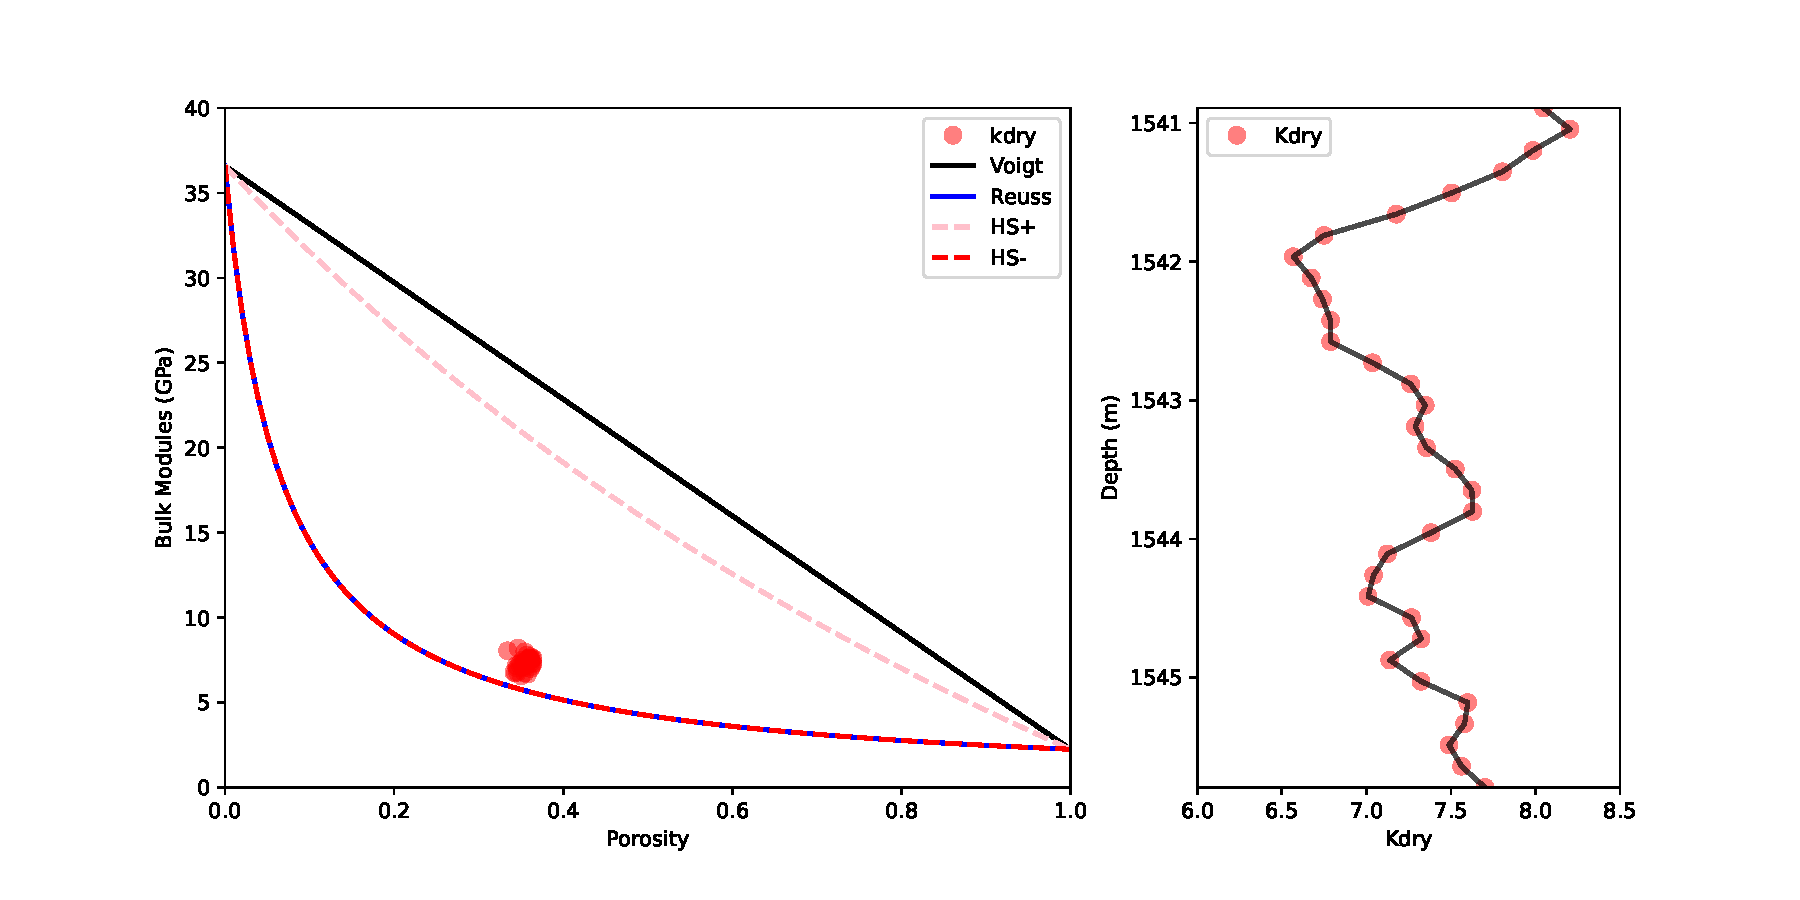
\includegraphics[width=0.8\textwidth]{figures/homework-1/p2-problem-1.pdf}
        \caption{The dry frame modulus ($K_{dry}$) for the reservoir interval}
        \label{fig:kdry}
    \end{figure}
\end{solution}


%%%%%%%%% T-2 %%%%%%%%%%
\begin{problem}{2}
    Derive the equation for grain density assuming fluid properties, porosity, and bulk density are known. Calculate the grain density for the reservoir interval from the given logs assuming 100\% brine saturation. Is the assumption that the mineral is only quartz grains reasonable? If not, what is the composition?
\end{problem}

\begin{solution}

    Derive the equation for grain density assuming fluid properties, porosity, 
    and bulk density are known, showing in formula ~\ref{equ:density}. 
    I get the result is a little different from the density of quartz, 
    so there are some other minerals whose density is smaller than quartz, for example clay.
    \begin{align}
        \rho_{min} &  = \frac{\rho - \phi * \rho_{brine}}{1-\phi}  \\
        &  = 2.634 (g/cc) \\
        \rho_{quartz} &  = 2.650 (g/cc)
        \label{equ:density}
    \end{align}
\end{solution}

%%%%%%%%% T-3 %%%%%%%%%%
\begin{problem}{3}
    Use Gassmann’s model and determine the formation V pand V safter 100\% scCO2 saturation. Plot the original logs and the property variations after full CO 2 saturation in the interval. See the table below for fluid property estimates.
\end{problem}

\begin{solution}

    I plot the original logs and the property variations after full CO2 saturation in the interval, $V_p, V_s, and \ \rho$ respectively.
    \begin{figure}[H]
        \centering
        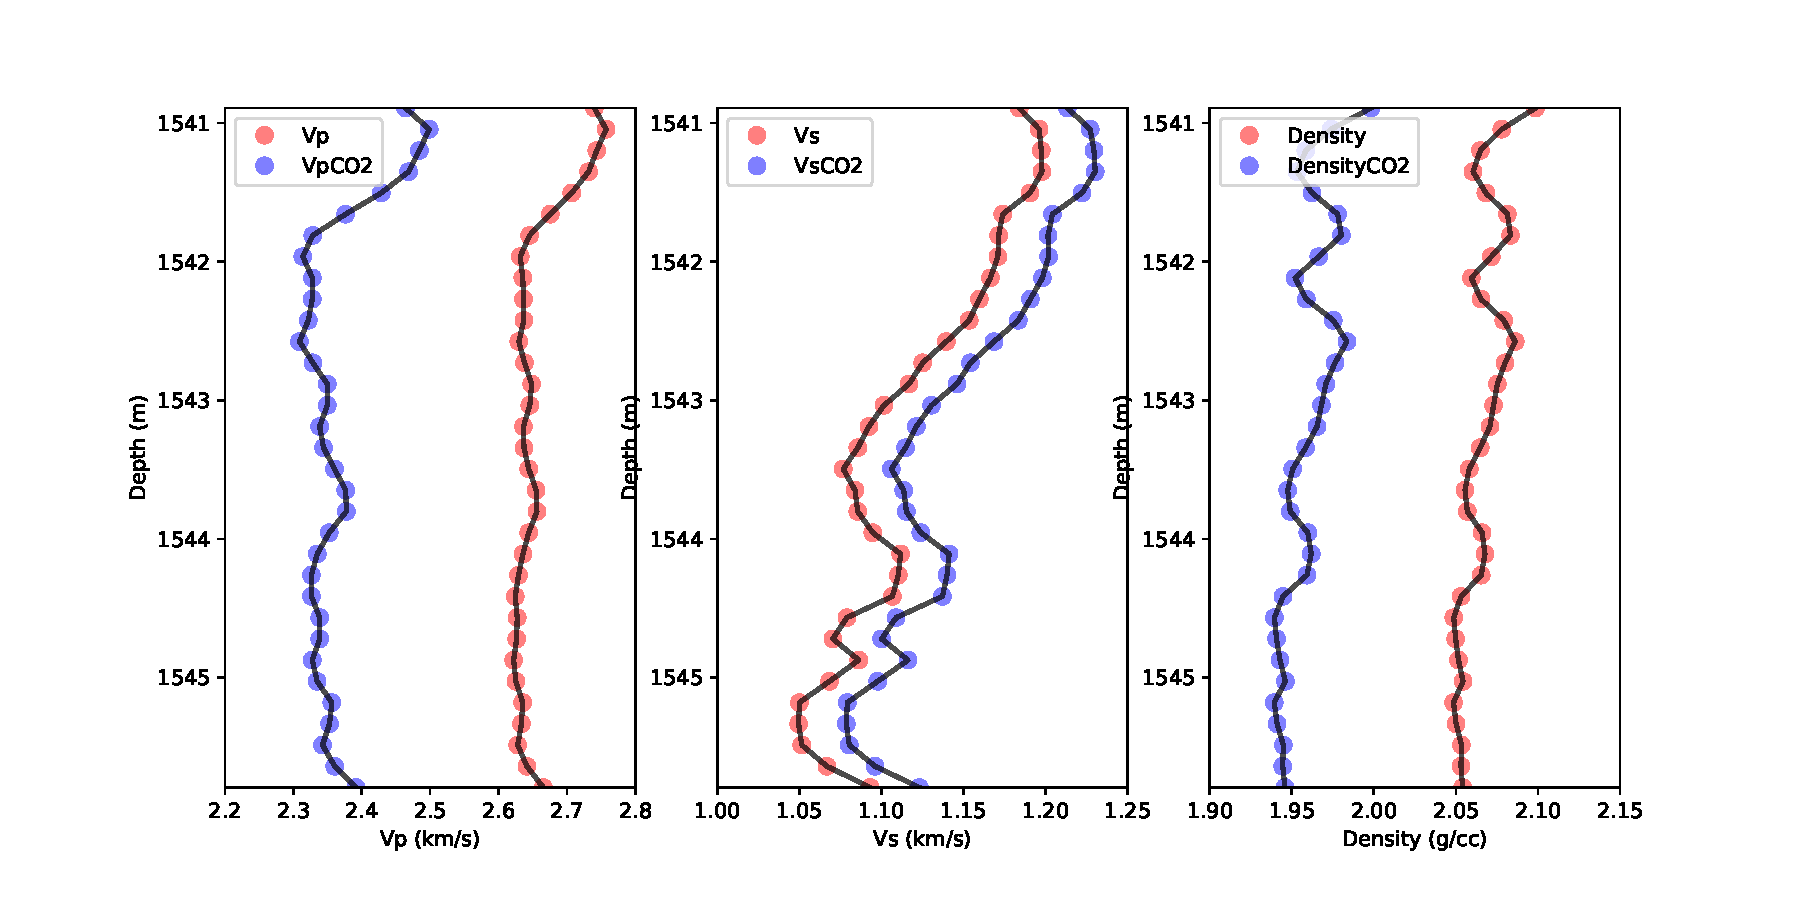
\includegraphics[width=0.8\textwidth]{figures/homework-1/p2-problem-3.pdf}
        \caption{The original logs and after $CO_2$ saturation logs}
        \label{fig:co2-saturation}
    \end{figure}
\end{solution}

%%%%%%%%% T-4 %%%%%%%%%%
\begin{problem}{4}
    Block the Vp, Vs, and density values for the CO 2saturated unit and the unit directly above. What is the change in normal P-wave reflectivity generated by CO 2 injection?
    Suggestions: Make 2 functions: the first calculates the dry rock bulk modulus, and the second computes the saturated-rock bulk modulus. Allow the functions to operate on vectors that are the length of the input curves. Fluid density, matrix density, and fluid bulk modulus should all be vectors. Make sure that your codes work. You will use this fluid substitution code again in later assignments (and quite possibly in your own work).
\end{problem}

\begin{solution}

    The defintion of reflectivity is showed in formula ~\ref{equ:reflectivity}
    \begin{align}
        reflectivity = \frac{(\rho_2*V_2 - \rho_1*V_1) }{ (\rho_2*V_2 + \rho_1*V_1)}
        \label{equ:reflectivity}
    \end{align}

    If we block the $V_p, V_s, and \ \rho$ for the $CO_2$ saturated, the reflectivity won't change in normal P-wave.
\end{solution}


%%%%%%%%%%%%%%%%%%%%%%%%%%%%%%%%%%%%%%%%%%%%%%%%%%%
%                  2. Part-2
%%%%%%%%%%%%%%%%%%%%%%%%%%%%%%%%%%%%%%%%%%%%%%%%%%%

\section{Scripts}
Noted: I transform jupyter-notebook to python scripts and show it here. 
If you want to run the scripts, I recommended to use original jupyter-notebook scripts instead of transformed python scripts. 

\subsection{Part-1}

% \begin{pythoncode}
%     import numpy as np
%     """
%         Annotation here.
%     """
%     # Annotation here.
%     def main():
%         for i in range(0,10,1):
%             if i == 1:
%                 print("Hello world")
    
%     # Annotation here.
%     if __name__ == "__main__":
%         main()
% \end{pythoncode}

\pythonfile{figures/homework-1/Part-1.py}
\subsection{Part-2}
\pythonfile{figures/homework-1/Part-2.py}
\clearpage